%% abtex2-modelo-trabalho-academico.tex, v-1.9.6 laurocesar
%% Copyright 2012-2016 by abnTeX2 group at http://www.abntex.net.br/ 
%%
%% This work may be distributed and/or modified under the
%% conditions of the LaTeX Project Public License, either version 1.3
%% of this license or (at your option) any later version.
%% The latest version of this license is in
%%   http://www.latex-project.org/lppl.txt
%% and version 1.3 or later is part of all distributions of LaTeX
%% version 2005/12/01 or later.
%%
%% This work has the LPPL maintenance status `maintained'.
%% 
%% The Current Maintainer of this work is the abnTeX2 team, led
%% by Lauro César Araujo. Further information are available on 
%% http://www.abntex.net.br/
%%
%% This work consists of the files abntex2-modelo-trabalho-academico.tex,
%% abntex2-modelo-include-comandos and abntex2-modelo-references.bib
%%

% ------------------------------------------------------------------------
% ------------------------------------------------------------------------
% abnTeX2: Modelo de Trabalho Academico (tese de doutorado, dissertacao de
% mestrado e trabalhos monograficos em geral) em conformidade com 
% ABNT NBR 14724:2011: Informacao e documentacao - Trabalhos academicos -
% Apresentacao
% ------------------------------------------------------------------------
% ------------------------------------------------------------------------

\documentclass[
	% -- opções da classe memoir --
	12pt,				% tamanho da fonte
	%openright,			% capítulos começam em pág ímpar (insere página vazia caso preciso)
	%twoside,			% para impressão em recto e verso. Oposto a oneside
	oneside,			% impressão de um lado só
	a4paper,			% tamanho do papel. 
	% -- opções da classe abntex2 --
	chapter=TITLE,		% títulos de capítulos convertidos em letras maiúsculas
	section=TITLE,		% títulos de seções convertidos em letras maiúsculas
	%subsection=TITLE,	% títulos de subseções convertidos em letras maiúsculas
	%subsubsection=TITLE,% títulos de subsubseções convertidos em letras maiúsculas
	sumario=tradicional % opção de sumário
	% -- opções do pacote babel --
	english,			% idioma adicional para hifenização
	french,				% idioma adicional para hifenização
	spanish,			% idioma adicional para hifenização
	brazil				% o último idioma é o principal do documento
	]{abntex2}

% ---
% Pacotes básicos 
% ---
\usepackage{lmodern}			% Usa a fonte Latin Modern			
\usepackage[T1]{fontenc}		% Selecao de codigos de fonte.
\usepackage[utf8]{inputenc}		% Codificacao do documento (conversão automática dos acentos)
\usepackage{lastpage}			% Usado pela Ficha catalográfica
\usepackage{indentfirst}		% Indenta o primeiro parágrafo de cada seção.
\usepackage{color}				% Controle das cores
\usepackage{graphicx}			% Inclusão de gráficos
\usepackage{microtype} 			% Melhorias de justificação
\usepackage{hyperref}
\usepackage{facens}				% Padrão Facens
\usepackage{pdfpages}			% Include de pdfs
\usepackage{lipsum}				% Geração de dummy text
\usepackage[alf]{abntex2cite}	% Citações padrão ABNT
%\usepackage[brazilian,hyperpageref]{backref}	 % Paginas com as citações na bibl
% ---

% ---
% Indicando pasta de figuras\\
% ---
\graphicspath{{imagens/}}
% ---

% --- 
% CONFIGURAÇÕES DE PACOTES
% --- 

% ---
% Configurações do pacote backref
% Usado sem a opção hyperpageref de backref
%\renewcommand{\backrefpagesname}{Citado na(s) página(s):~}
% Texto padrão antes do número das páginas
%\renewcommand{\backref}{}
% Define os textos da citação
%\renewcommand*{\backrefalt}[4]{
%	\ifcase #1 %
%		Nenhuma citação no texto.%
%	\or
%		Citado na página #2.%
%	\else
%		Citado #1 vezes nas páginas #2.%
%	\fi}%
% ---

%VARIAVEIS
%---

%---
% ---
% Informações de dados para CAPA e FOLHA DE ROSTO
% ---
\titulo{RELATÓRIO DE ESTÁGIO SUPERVISIONADO OBRIGATÓRIO}
\autor{Alex Covolan Vieira Coelho}
\local{Sorocaba/SP}
\data{2017}
\orientador[Dra.]{Andrea Vieira Braga}
\instituicao{Faculdade de Engenharia de Sorocaba - FACENS}
\tipotrabalho{Dissertação}

% O preambulo deve conter o tipo do trabalho, o objetivo, 
% o nome da instituição e a área de concentração 
\preambulo{Relatório apresentado como requisito obrigatório para a integralização do Curso de Engenharia da Computação.}
% ---

%---
% Lista de figuras contando por seção
%---
%\counterwithin{figure}{section}

% ---
% Configurações de aparência do PDF final

% alterando o aspecto da cor azul
\definecolor{blue}{RGB}{41,5,195}

% informações do PDF
\makeatletter
\hypersetup{
     	%pagebackref=true,
		pdftitle={\@title}, 
		pdfauthor={\@author},
    	pdfsubject={\imprimirpreambulo},
	    pdfcreator={LaTeX with abnTeX2},
		pdfkeywords={abnt}{latex}{abntex}{abntex2}{trabalho acadêmico}, 
		colorlinks=false,       		% false: boxed links; true: colored links
    	linkcolor=blue,          	% color of internal links
    	citecolor=blue,        		% color of links to bibliography
    	filecolor=magenta,      		% color of file links
		urlcolor=blue,
		bookmarksdepth=4
}
\makeatother
% --- 

% --- 
% Espaçamentos entre linhas e parágrafos 
% --- 

% O tamanho do parágrafo é dado por:
\setlength{\parindent}{1.25cm}

% Controle do espaçamento entre um parágrafo e outro:
\setlength{\parskip}{0.2cm}  % tente também \onelineskip

% ---
% compila o indice
% ---
\makeindex
% ---

% ----
% Início do documento
% ----
\begin{document}
% Seleciona o idioma do documento (conforme pacotes do babel)
%\selectlanguage{english}
\selectlanguage{brazil}

% Retira espaço extra obsoleto entre as frases.
\frenchspacing 

% ----------------------------------------------------------
% ELEMENTOS PRÉ-TEXTUAIS
% ----------------------------------------------------------
\pretextual

%\includepdf{report4.pdf}


% ---
% Capa
% ---
\imprimircapa
% ---

% ---
% Folha de rosto
% (o * indica que haverá a ficha bibliográfica)
% ---
\imprimirfolhaderosto*
% ---

% ---
% Inserir a ficha bibliografica
% ---

% Isto é um exemplo de Ficha Catalográfica, ou ``Dados internacionais de
% catalogação-na-publicação''. Você pode utilizar este modelo como referência. 
% Porém, provavelmente a biblioteca da sua universidade lhe fornecerá um PDF
% com a ficha catalográfica definitiva após a defesa do trabalho. Quando estiver
% com o documento, salve-o como PDF no diretório do seu projeto e substitua todo
% o conteúdo de implementação deste arquivo pelo comando abaixo:
%
% \begin{fichacatalografica}
%     \includepdf{fig_ficha_catalografica.pdf}
% \end{fichacatalografica}

%\include{pre-textuais/fichacatalografica}
% ---

% ---
% Inserir errata
% ---
%\include{pre-textuais/errata}
% ---

% ---
% Inserir folha de aprovação
% ---

% Isto é um exemplo de Folha de aprovação, elemento obrigatório da NBR
% 14724/2011 (seção 4.2.1.3). Você pode utilizar este modelo até a aprovação
% do trabalho. Após isso, substitua todo o conteúdo deste arquivo por uma
% imagem da página assinada pela banca com o comando abaixo:
%
% \includepdf{folhadeaprovacao_final.pdf}
%
%\include{pre-textuais/folhaaprovacao}
% ---

% ---
% Dedicatória
% ---
%\include{pre-textuais/dedicatoria}
% ---

% ---
% Agradecimentos
% ---
%\include{pre-textuais/agradecimentos}
% ---

% ---
% Epígrafe
% ---
%\include{pre-textuais/epigrafe}
% ---

% ---
% RESUMOS
% ---

% resumo em português
%\include{pre-textuais/resumo/pt_Br}

% resumo em inglês
%\include{pre-textuais/resumo/en}

% ---

% ---
% inserir lista de ilustrações
% ---
\include{pre-textuais/lista-ilustracoes}
% ---

% ---
% inserir lista de tabelas
% ---
%\include{pre-textuais/lista-tabelas}
% ---

% ---
% inserir lista de abreviaturas e siglas
% ---
\begin{siglas}
  \item[CRTSE] Centro Regional de Tecnologia Santa Escolástica
  \item[CRTS] Companhia Rede Telefônica Sorocabana
  \item[ACRTS] Associação Cultural de Renovação Tecnológica Sorocabana
  \item[IPEAS] Instituto de Pesquisas e Estudos Avançados Sorocabano
  \item[LEMAT] Laboratório de Ensaio de Materiais
  \item[ABMES] Associação Brasileira de Mantenedoras de Ensino Superior
\end{siglas}
% ---

% ---
% inserir lista de símbolos
% ---
%\include{pre-textuais/lista-simbolos}
% ---

% ---
% inserir o sumario
% ---
\include{pre-textuais/sumario}
% ---



% ----------------------------------------------------------
% ELEMENTOS TEXTUAIS
% ----------------------------------------------------------
\textual
% ---
\pagestyle{simple}


\chapter{Introdução}
\label{chap:cap1}
O presente relatório de estágio é elaborado como documento obrigatório para a conclusão do curso de Engenharia da Computação, apresentando as atividades realizadas durante as 360 horas de estágio, cumpridas dentro da Faculdade de Engenharia de Sorocaba (Facens). Mais especificamente atuando dentro do Laboratório de Informática, nos primeiros meses trabalhando com suporte aos computadores presentes na faculdade, além de atendimento \textit{help desk} e posteriormente trabalhando com desenvolvimento de aplicações WEB em PHP as quais serviram para atender as demandas da própria faculdade, tanto no âmbito corporativo como no educacional.

Tal estágio também proporcionou uma posterior contratação ao término dos 2 anos previsto em contrato, e este é o período considerado neste documento, pois após a contratação as áreas de atuação foram ampliadas, garantindo sólidos conhecimentos em novas tecnologias e plataformas, como Ruby, C\# e a plataforma Sales Force, compreendendo o período de maior aprendizado durante esta jornada. 

Mesmo com as novas tecnologias e áreas de atuação, a maior parte das aplicações a serem criadas continuaram sendo em PHP, além de dar suporte as aplicações antigas. Foi possível também aprender sobre a área de infraestrutura, passando a desempenhar a função de \textit{devops} e trabalhando ao lado dos analistas de redes.

Dentre os feitos durante o estágio, destaca-se a doação de um sistema de inscrições para a FUNDEC (Fundação de Desenvolvimento Cultural de Sorocaba), tal sistema agilizou a inscrição e processo de seleção de mais de 4 mil candidatos, os quais eram cadastrados na mão anteriormente, também é possível enunciar a colaboração no desenvolvimento de uma \textit{framework} própria desenvolvida dentro da FACENS pelo Eng. Flávio Bogila a qual ganhou o nome de "Bogila Framework", através dela possibilitou-se criar novas aplicações com maior velocidade devido ao fato dela já possuir \textit{templates} padrões, geração de código e uma arquitetura que facilitam seu uso nas aplicações da Faculdade.

\chapter{Plano de Estágio}
\label{chap:cap2}
Informações sobre a empresa e o estagiário são apresentados nesta seção.
\section{Identificação do Aluno}
\label{sec:identaluno}
\textbf{Nome:} Alex Covolan Vieira Coelho\\
\indent \textbf{Matrícula: } 132115\\
\indent \textbf{Curso: } Engenharia da Computação\\
\indent \textbf{Semestre: } 10º\\
\indent \textbf{Ano de ingresso: } 2013\\
\indent \textbf{E-mail: } alexcvcoelho@gmail.com\\

\section{Empresa}
\label{sec:empresa}
\textbf{Nome:} FACENS - Faculdade de Engenharia de Sorocaba \\
\indent \textbf{Razão Social:} Associacao Cultural de Renovacao Tecnologica Sorocabana \\
\indent \textbf{CNPJ:} 45.718.988/0003-29 \\
\indent \textbf{Área de atuação:} Educação superior\\
\indent \textbf{Endereço:} Rodovia Senador José Ermírio de Moraes, 1425 \\
\indent \textbf{Bairro:} Castelinho km 1,5 - Alto da Boa Vista \\
\indent \textbf{CEP:} 18087-125 \\
\indent \textbf{Cidade:} Sorocaba \\
\indent \textbf{Estado:} São Paulo \\
\indent \textbf{Nome do responsável pelos estágios na empresa:} João Alex Ramon \\
\indent \textbf{Telefone da área responsável pelos estágios:} (15) 3238-1188/216 \\

\begin{figure}[htb]
\caption{\label{fig:mapsfacens} Localização da Facens}
\begin{center}
\includegraphics[scale=0.65]{MapsFacens}
\end{center}
\end{figure}

\section{Estágio}
\label{sec:estagio}
\textbf{Área de atuação:} Desenvolvimento \\
\indent \textbf{Setor:} Tecnologia da Informação \\
\indent \textbf{Data de início de estágio:} \\
\indent \textbf{Data do fim de estágio:} \\
\indent \textbf{Período do dia que estagia:} Manhã e Tarde \\
\indent \textbf{Carga horária semanal:} 40 horas \\

\section{Supervisor de Estágio na Empresa}
\label{sec:supestagioempre}
\textbf{Nome:} Luis Gustavo Martins Monteiro \\
\indent \textbf{Formação acadêmica:} \\
\indent \indent Especialização em Redes de Computadores, UNICAMP, 2006 \\
\indent \indent Graduação em Sistemas de Informação, Uirapuru Superior, 2005 \\
\indent \textbf{Cargo:} Coordenador da Tecnologia da Informação \\
\indent \textbf{Departamento:} Tecnologia da Informação \\
\indent \textbf{Responsabilidades do departamento:} Desenvolvimento e suporte de soluções tecnológicas \\
\indent \textbf{Telefone:} (15) 3238-1188/236 \\
\indent \textbf{E-mail:} gustavo.monteiro@facens.br \\

\section{Atividades Programadas Para o Estagiário}
\label{sec:ativestagiario}


\chapter{Organograma da Empresa}
\label{chap:chap3}
\textbf{Diretor:} \\ \indent Eng. Paulo Roberto Freitas de Carvalho \\
\indent paulo.carvalho@facens.br \\

\textbf{Vice Diretor:} \\ \indent  Prof. Dr. Fabiano Prado Marques \\
\indent fabiano.marques@facens.br \\

\textbf{Coordenação Engenharia Civil:}\\ \indent  Prof. Dr. José Antonio De Milito \\
\indent jose.milito@facens.br \\

\textbf{Coordenação Engenharia da Computação:}\\ \indent Prof.ª Dra. Andréa Lucia Braga Vieira Rodrigues \\
\indent andrea.braga@facens.br \\

\textbf{Coordenação Engenharia Elétrica:} \\ \indent Prof. Dr. Anderson Marcos Henriques \\
\indent anderson.henriques@facens.br \\

\textbf{Coordenação Engenharia Mecânica:} \\ \indent Prof. Dr. Francisco Scinocca \\
\indent francisco.scinocca@facens.br \\

\textbf{Coordenação Engenharia Mecatrônica:} \\ \indent Prof. Dr. Anderson Marcos Henriques \\
\indent anderson.henriques@facens.br \\

\textbf{Coordenação Engenharia Produção:} \\ \indent Prof. Dr. José Lázaro Ferraz \\
\indent jose.ferraz@facens.br \\

\textbf{Coordenação Engenharia Química:} \\ \indent Prof.ª Dra. Sandra Bizarria Lopes Villanueva \\
\indent sandra.lopes@facens.br \\

\textbf{Coordenação Tecnologia em Jogos Digitais:} \\ \indent Prof.ª Dra. Andréa Lucia Braga Vieira Rodrigues \\
\indent andrea.braga@facens.br \\

\textbf{Coordenação Engenharia Agronômica:} \\ \indent Prof.ª Me. Thais Prado Avancini \\
\indent thais.avancini@facens.br \\

\textbf{Coordenação Engenharia de Alimentos:} \\ \indent Prof. Dra. Cláudia Maria Treumann Rocha \\
\indent claudia.treumann@facens.br \\

\textbf{Coordenação Acadêmica:} \\ \indent Prof.ª Dra. Sandra Bizarria Lopes Villanueva \\
\indent sandra.lopes@facens.br \\

\textbf{Coordenação Ciclo Básico:} \\ \indent Prof. Me. Marcos Vinícius Ribeiro \\
\indent marcos.ribeiro@facens.br \\

\textbf{Coordenação de projetos:}  \\

\textbf{Smart Campus Facens:} \\ \indent Prof.ª Dra. Regiane Relva Romano \\
\indent regiane.relva@facens.br \\

\textbf{Fab Lab Facens:} \\ \indent Siron Cesar Paccheco Pereira \\
\indent siron.pereira@facens.br \\

\textbf{LIGA Facens:} \\ \indent Prof. Wilson Roberto Marcondes de Oliveira Junior \\
\indent wilson.junior@facens.br \\

\textbf{Pós, Extensão e Cursinho Pré-Vestibular:} \\ \indent Prof. Dr. Adriano Pila \\
\indent adriano.pila@facens.br \\

\textbf{Facens Tech (IPEAS/LEMAT/LIGA):} \\ \indent Prof. Me. Antonio Carlos Gomes \\
\indent antonio.gomes@facens.br \\

\textbf{Farm Lab Facens:} \\ \indent Prof.ª Me. Thais Prado Avancini \\
\indent thais.avancini@facens.br \\

\textbf{FACE (Facens Centro de Empreendedorismo):} \\ \indent Prof.ª Me. Andréia Damasio Leles \\
\indent andrea.leles@facens.br

\section{A Empresa}
\label{sec:aempresa}
\begin{figure}[htb]
	\caption{\label{fig:mapsfacens} Faixada da Facens}
	\begin{center}
		\includegraphics[scale=0.85]{facensfachada}
	\end{center}
\end{figure}

A Faculdade de Engenharia de Sorocaba - Facens - teve como embrião a Companhia Rede Telefônica Sorocabana ( CRTS ) responsável pelo sistema de telefonia de toda região sorocabana, em meados dos anos 70. A necessidade de profissionais capacitados para atuar no setor de telecomunicações fez com que a CRTS criasse, em 1974, o Centro Regional de Tecnologia Santa Escolástica ( CRTSE ), mais conhecido como Colégio da Engenharia. Os cursos de Telecomunicações e Eletrônica foram os primeiros a ser ministrados pelo colégio técnico - em salas cedidas pelo Colégio Santa Escolástica.

O rápido desenvolvimento do setor de telecomunicações na região fez com que a mão de obra especializada se tornasse imprescindível. No mesmo ano de implantação do Colégio, a Associação Cultural de Renovação Tecnológica Sorocabana (ACRTS) - mantenedora do Colégio da Engenharia e da Facens - protocolou no Ministério de Educação e Cultura (MEC) um pedido para instalação da Faculdade de Engenharia na cidade de Sorocaba. Em outubro de 1976, foi publicada a autorização para a implantação dos primeiros cursos da Faculdade, de Engenharia Civil e Engenharia Elétrica os quais tiveram seus vestibulares abertos em janeiro de 1977, que passaram a funcionar no 3º andar do Instituto de Educação Ciências e Letras.

Em 1978, foram iniciadas as construções do campus universitário da Faculdade criada para suprir uma grave lacuna no Ensino Superior de Sorocaba. Em 03 de junho de 1980, a Facens foi reconhecida pelo MEC. A construção do campus foi concluída em 1984 com a implantação dos prédios de Engenharia Civil e Elétrica, laboratórios para esses cursos e o ginásio de esportes.
Em anos mais recentes, a Facens recebeu autorização para ministrar os cursos de Engenharia da Computação (1998) e de Engenharia Mecânica (2001) atendendo assim, à crescente demanda por tais profissionais na Região. Por este mesmo motivo passou a oferecer, no final da década de 90, cursos de Especialização e Pós-Graduação Lato-Sensu.

Em 1991 a Semana da Engenharia foi incluída no calendário acadêmico, passando a expor projetos de alunos durante três dias a todos da comunidade, além de proporcionar cursos e palestras para os alunos. Em 2001 a Facens passou a oferecer o curso de Engenharia Mecânica reconhecido pelo MEC, a fim de capacitar profissionais para o Parque Tecnológico da região. No mesmo ano o IPEAS (Instituto de Pesquisas e Estudos Avançados Sorocabano) começou suas atividades dentro do campus, prestando serviços a empresas da região na área tecnológica. Em 2003 o LEMAT (Laboratório de Ensaio de Materiais) deixou de atuar apenas como laboratório acadêmico, passando a prestar serviços para empresas da região.

Em 2004 iniciou-se o Cursinho Pré-Vestibular com a intenção de nivelar o conhecimento de alunos da rede pública e privada para ingresso nas instituições de ensino superior. Em 2005 foi realizada a 1ª Maratona de Programação O evento é uma competição interna que a faculdade promove seguindo os moldes da Maratona de Programação da Sociedade Brasileira de Computação (Regional Sulamericana do Concurso da ACM). A maratona é um torneio onde equipes formadas por alunos devem resolver problemas computacionais, utilizando conhecimentos técnicos, criatividade, capacidade de trabalho em equipe e habilidade de resolver problemas sob pressão.

Em 2008 é realizada a 1ª Maratona de Desenvolvimento de Jogos. A Maratona de Desenvolvimento de Jogos da Facens é um concurso técnico e cultural que busca incentivar o estudo e a aplicação das tecnologias que envolvem o desenvolvimento de jogos eletrônicos por parte dos alunos da Faculdade.

Em 2010 é aberto o curso de Engenharia Mecatrônica. Em 2011 é dado início a Construção do Prédio C. Nos 7 mil metros quadrados de construção são mais 30 salas de aula, todas equipadas com lousas digitais, sistema de som e adequações acústicas. Com estrutura pré-montada e linhas arquitetônicas modernas, além de utilizar toda a tecnologia disponível, existe também a preocupação com sustentabilidade.

\begin{figure}[htb]
	\caption{\label{fig:predioc} Prédio C}
	\begin{center}
		\includegraphics[scale=0.3]{predioc}
	\end{center}
\end{figure}

Em 2012 é aberto o curso de Engenharia de Produção e Engenharia Química. Em 2014 é lançado o Smart Campus Facens com o objetivo de  desenvolver, implementar, testar, analisar e replicar soluções para Cidades Inteligentes, utilizando o campus universitário como uma área para estudos das soluções que possam ser replicadas nas cidades. Prioriza-se a transformação de problemas reais em soluções aplicáveis no contexto urbano, alinhando-as com as necessidades, crises e desafios do Brasil para as próximas décadas. 

Em 2015 iniciou-se o curso de Tecnologia de Jogos Digitais, o primeiro curso tecnólogo dentro da Facens. No mesmo ano ocorreu a inauguração do Fab Lab Facens, o primeiro laboratório de prototipação no interior de São Paulo, o Fab Lab Facens é um laboratório de fabricação digital pertencente à rede mundial Fab Lab, criada pelo MIT com o objetivo de facilitar a prototipagem de ideias e visando a inovação e invenção. Onde estudantes, educadores, empresas, profissionais, inventores, curiosos e especialistas podem adquirir conhecimento, trocar experiências e utilizar equipamentos para tornar seus projetos em realidade.

Em 2016 iniciou-se o curso de Engenharia de Alimentos e Engenharia Agronômica. No mesmo ano a Facens ganhou o Prêmio Top Educacional através do programa Smart Campus da Facens, concedido pela Associação Brasileira de Mantenedoras de Ensino Superior (ABMES).

A Facens conta com um destacado corpo docente, a nível acadêmico e profissional, bem como com uma infraestrutura de qualidade suportada por laboratórios muito bem equipados e tecnologicamente atualizados. Esses fatores são decisivos para o reconhecimento ao trabalho pedagógico que a Faculdade desenvolve e, principalmente, à qualidade dos profissionais aqui formados.

Mantida pela ACRTS, uma entidade de Utilidade Pública Federal sem fins lucrativos e certificada como filantrópica pelo Conselho Nacional de Assistência Social, concede inúmeras bolsas de estudos aos seus alunos que apresentam carência socioeconômica comprovada e investe todo o seu resultado em prol da Faculdade, o que possibilita à Facens ser um centro educacional em constante evolução.

\section{Objeto de Produção da Empresa e Missão}
\label{sec:prodmissaoempresa}
A Faculdade de Engenharia de Sorocaba (FACENS) tem como missão: "Formar cidadãos capacitados, felizes, responsáveis, empreendedores, inovadores e capazes de criar soluções tecnológicas, sustentáveis e que transformem a sociedade".

\begin{enumerate}
	\item Estimular a criação cultural e o desenvolvimento do espírito científico e do pensamento reflexivo;
	\item Formar diplomados nas diferentes áreas de conhecimento, aptos para a inserção em setores profissionais e para a participação no desenvolvimento da sociedade brasileira, e colaborar na sua formação contínua;
	\item Incentivar o trabalho de pesquisa e investigação científica, visando o desenvolvimento da ciência e da tecnologia e da criação e difusão da cultura, e, desse modo, desenvolver o entendimento do homem e do meio em que vive;
	\item Promover a divulgação de conhecimentos culturais, científicos e técnicos que constituem patrimônio da humanidade e comunicar o saber através do ensino, de publicações ou de outras formas de comunicação;
	\item Suscitar o desejo permanente de aperfeiçoamento cultural e profissional e possibilitar a correspondente concretização, integrando os conhecimentos que vão sendo adquiridos numa estrutura intelectual sistematizadora do conhecimento de cada geração;
	\item Estimular o conhecimento dos problemas do mundo presente, em particular os nacionais e regionais, prestar serviços especializados à comunidade e estabelecer com esta uma relação de reciprocidade;
	\item Promover a extensão, aberta à participação da população, visando à difusão das conquistas e benefícios resultantes da criação cultural e da pesquisa científica e tecnológica geradas na instituição.
\end{enumerate}

\section{Organograma do Setor}
\label{sec:aempresa}
\textbf{Coordenadora de TI do grupo Splice:} \\ \indent  Heloísa Helena Camilo \\
\indent heloisa.camilo@facens.br \\

\textbf{Coordenador de Infraestrutura do grupo Splice:} \\ \indent Rodolfo Belloti \\
\indent rodolfo.belloti@facens.br \\

\textbf{Coordenador de TI da Facens:} \\ \indent Luis Gustavo Monteiro \\
\indent gustavo.monteiro@facens.br \\

\textbf{Analista Sênior:} \\ \indent Lucas Alves da Mota \\
\indent lucas.mota@facens.br \\

\textbf{Analista de Sistemas Júnior:} \\ \indent  Diogo Silva \\
\indent diogo.silva@facens.br \\

\textbf{Analista de Redes Júnior:} \\ \indent  Tiago Barbosa Ferreira \\
\indent tiago.barbosa@facens.br \\

\textbf{Analista de Redes Pleno:} \\ \indent  Renato Bonani \\
\indent renato.bonani@facens.br \\

\textbf{Analista de Sistemas Pleno:} \\ \indent  Flavio Bogila \\
\indent flavio.bogila@facens.br \\

\textbf{Analista de Sistemas Júnior:} \\ \indent  Alex Covolan Vieira Coelho \\
\indent alex.coelho@facens.br \\

\section{Atribuições do Setor}
\label{sec:atribsetor}
O setor é compreendido em duas áreas, uma relacionada com infraestrutura e a outra com sistemas e desenvolvimento. Na área de infraestrutura se tem os analistas de rede e os analistas de suporte os quais trabalham em conjunto para manter o funcionamento da rede interna e a disponibilidade dos sistemas que rodam em servidores internos, além da telefonia Voip, bem como manter os computadores, tanto corporativos como educacionais, em perfeito funcionamento para que o usuário, sendo ele funcionário ou aluno possa desempenhar seu trabalho, nestes são aplicados regras de acesso limitando determinados tipos de acesso aos computadores, como bloqueios de USB e restrições a determinados sites. É por parte deles também a responsabilidade de realizar a instalação de novos softwares e manter as licenças dos mesmos atualizadas, tanto para o uso dos trabalhadores como para os alunos em sala de aula.

A área relacionada com sistemas trabalha dentro da plataforma Totvs a fim de manter os dados dos alunos e funcionários, e através dessa base de dados a área de desenvolvimento consome os dados para criação de aplicações úteis tanto para funcionários como para alunos. Estas aplicações na área acadêmica vão desde sistemas para troca de email e senha como sistemas de inscrições para maratonas   e eventos dentro da faculdade.

Dentre os sistemas desenvolvidos e mantidos pelo setor podem ser citados o de agendamentos para o Fab Lab, lista de consulta de contatos, inscrições para TecnoFacens, pedidos de licença de software, sistema de chamadas, sistema de histórico, sistema de monitoria, sistema de controle para descontar créditos e alterar senha, além de APIs para serem consumidas por aplicações de terceiros, principalmente APIs para login no servidor de AD através de LDAP.

Entre outras responsabilidades do setor está o de garantir a proteção e consistência dos dados que estão sob domínio do setor, para isso dentro da arquitetura de infra existem servidores os quais armazenam \textit{backups} diários do banco de dados, além de \textit{snapshots} das máquinas virtuais. Desta forma os dados estão protegidos contra catástrofes, e os servidores que armazenam os dados e \textit{backups} estão localizados em um CPD com gerador de energia para períodos de falta de energia.

\section{Processo de Seleção}
\label{sec:procselecao}
O processo de seleção foi compreendido em etapa única, a qual na época era para uma vaga de estagiário como atendente no \textit{help desk} e também para dar suporte aos computadores da faculdade, prestando atendimento primeiro nível aos analistas de suporte, um estágio de 6 horas diárias no período da tarde, recebendo bolsa estágio. 

Os entrevistadores eram os analistas de redes, na época o Eng. Bruno Rodrigues e o Eng. Alexandre Machado, que após a entrevista me informaram que fui selecionado para a vaga, e então passei a desempenhar esta função por três meses. Logo depois os mesmos recrutadores me ofereceram estágio como desenvolvedor, mesmo eu não tendo experiência na época, aceitei e passei a atuar no desenvolvimento de software inicialmente apenas com PHP, trabalhando diretamente ao lado do Eng. Flávio Bogila e Eng. Alexandre Machado, além do estagiário Guilherme Pannayotou que desempenhava a função de \textit{front-end}, enquanto eu trabalhava no \textit{backend} das aplicações.

Ao término dos dois anos de contrato de estágio recebi o convite para trabalhar no cargo de Analista de Sistemas Júnior em regime CLT, agora trabalhando no time de desenvolvimento composto por mim e o Eng. Flávio, expandindo os conhecimentos para Ruby, C\# e Apex presente na plataforma SalesForce a qual passou-se a utilizar dentro da empresa. Nesta nova função todas as atividades desenvolvidas englobam trabalho em equipe ao lado do time de infraestrutura e sistemas, pois para manter os sistemas no ar era preciso de recursos de servidores e também precisam ser alimentados com dados presentes no sistema Totvs, no qual está todas as informações dos usuários. 

\chapter{Recursos disponíveis}
\label{chap:chap4}
Entre os recursos disponíveis estão computadores atuais, conectados a uma internet de alta qualidade com links dedicados e auxiliares.

\section{Recursos do Estágio}
A sala do TI, na qual se realizou o estágio está situada no prédio E dentro da faculdade, no segundo andar (andar administrativo), as salas são equipadas com uma máquina para cada colaborador, sendo a minha em questão com processador i7 e 8 GB de memória RAM, mostrado na figura \ref{fig:pc}, possibilitando desenvolver e testar todo o tipo de tecnologia referente a desenvolvimento

\subsection{Linux}
Utilizou-se o sistema operacional Linux para maior facilidade na instalação e configuração das tecnologias utilizadas durante o estágio, se utilizando da distribuição Linux Mint versão 17.0 (Sarah) com interface gráfica Cinamon, como mostrado na figura \ref{fig:linux}. Isto só foi possível através da política da empresa que permitiu o uso de um sistema operacional diferente ao do padrão adotado pela faculdade, que é o Windows.

\begin{figure}[htb]
	\caption{\label{fig:linux} Linux Mint}
	\begin{center}
		\includegraphics[scale=0.3]{linux}
	\end{center}
\end{figure}


\section{Oficinas e Laboratórios}
\label{sec:oficlabs}
A Facens conta com 9 prédios, em que neles estão laboratórios destinados a alunos, sendo que cada curso se utiliza de um conjunto de laboratórios, como por exemplo o curso de Engenharia de Computação, o qual utiliza os laboratórios de Química, Informática e Elétrica, além das salas de aulas. Todos os laboratórios e salas de aulas são equipadas com projetores e lousas digitais, as quais proporcionam um ótimo aprendizado ao aluno, mantendo a sua excelência no ensino.

\subsection{Laboratório de Informática}
Um dos 9 prédios da Faculdade é onde está localizado o Laboratório de Informática (LI), o qual possui dentro dele 13 salas equipadas com computadores e projetores, utilizados durante as aulas, nos computadores é possível encontrar \textit{softwares} acadêmicos os quais atendem as demandas de todos os cursos, possibilitando o desenvolvimento de projetos acadêmicos, além de permitir aos alunos acesso a \textit{internet}.

É dentro do LI que se encontra também toda a equipe de suporte responsável pela manutenção, e mantimento de todas as máquinas presentes na Faculdade, além das próprias contidas no LI, dentre essas máquinas estão também as impressoras utilizadas por todos os setores. Juntamente com a equipe do LI trabalha o setor de Tecnologia da Informação (TI) o qual tem a responsabilidade de desenvolver e manter sistemas tanto corporativos como acadêmicos em funcionamento, além de cuidar de toda a infraestrutura de rede presente na faculdade.

Dentro do LI os alunos tem a oportunidade de enriquecer seu aprendizado através de aulas práticas, desfrutando de ferramentas onlines ou \textit{softwares} licenciados para estudantes.

\subsection*{Laboratório de Elétrica}

\begin{figure}[htb]
	\caption{\label{fig:eletrica} Laboratório de Elétrica}
	\begin{center}
		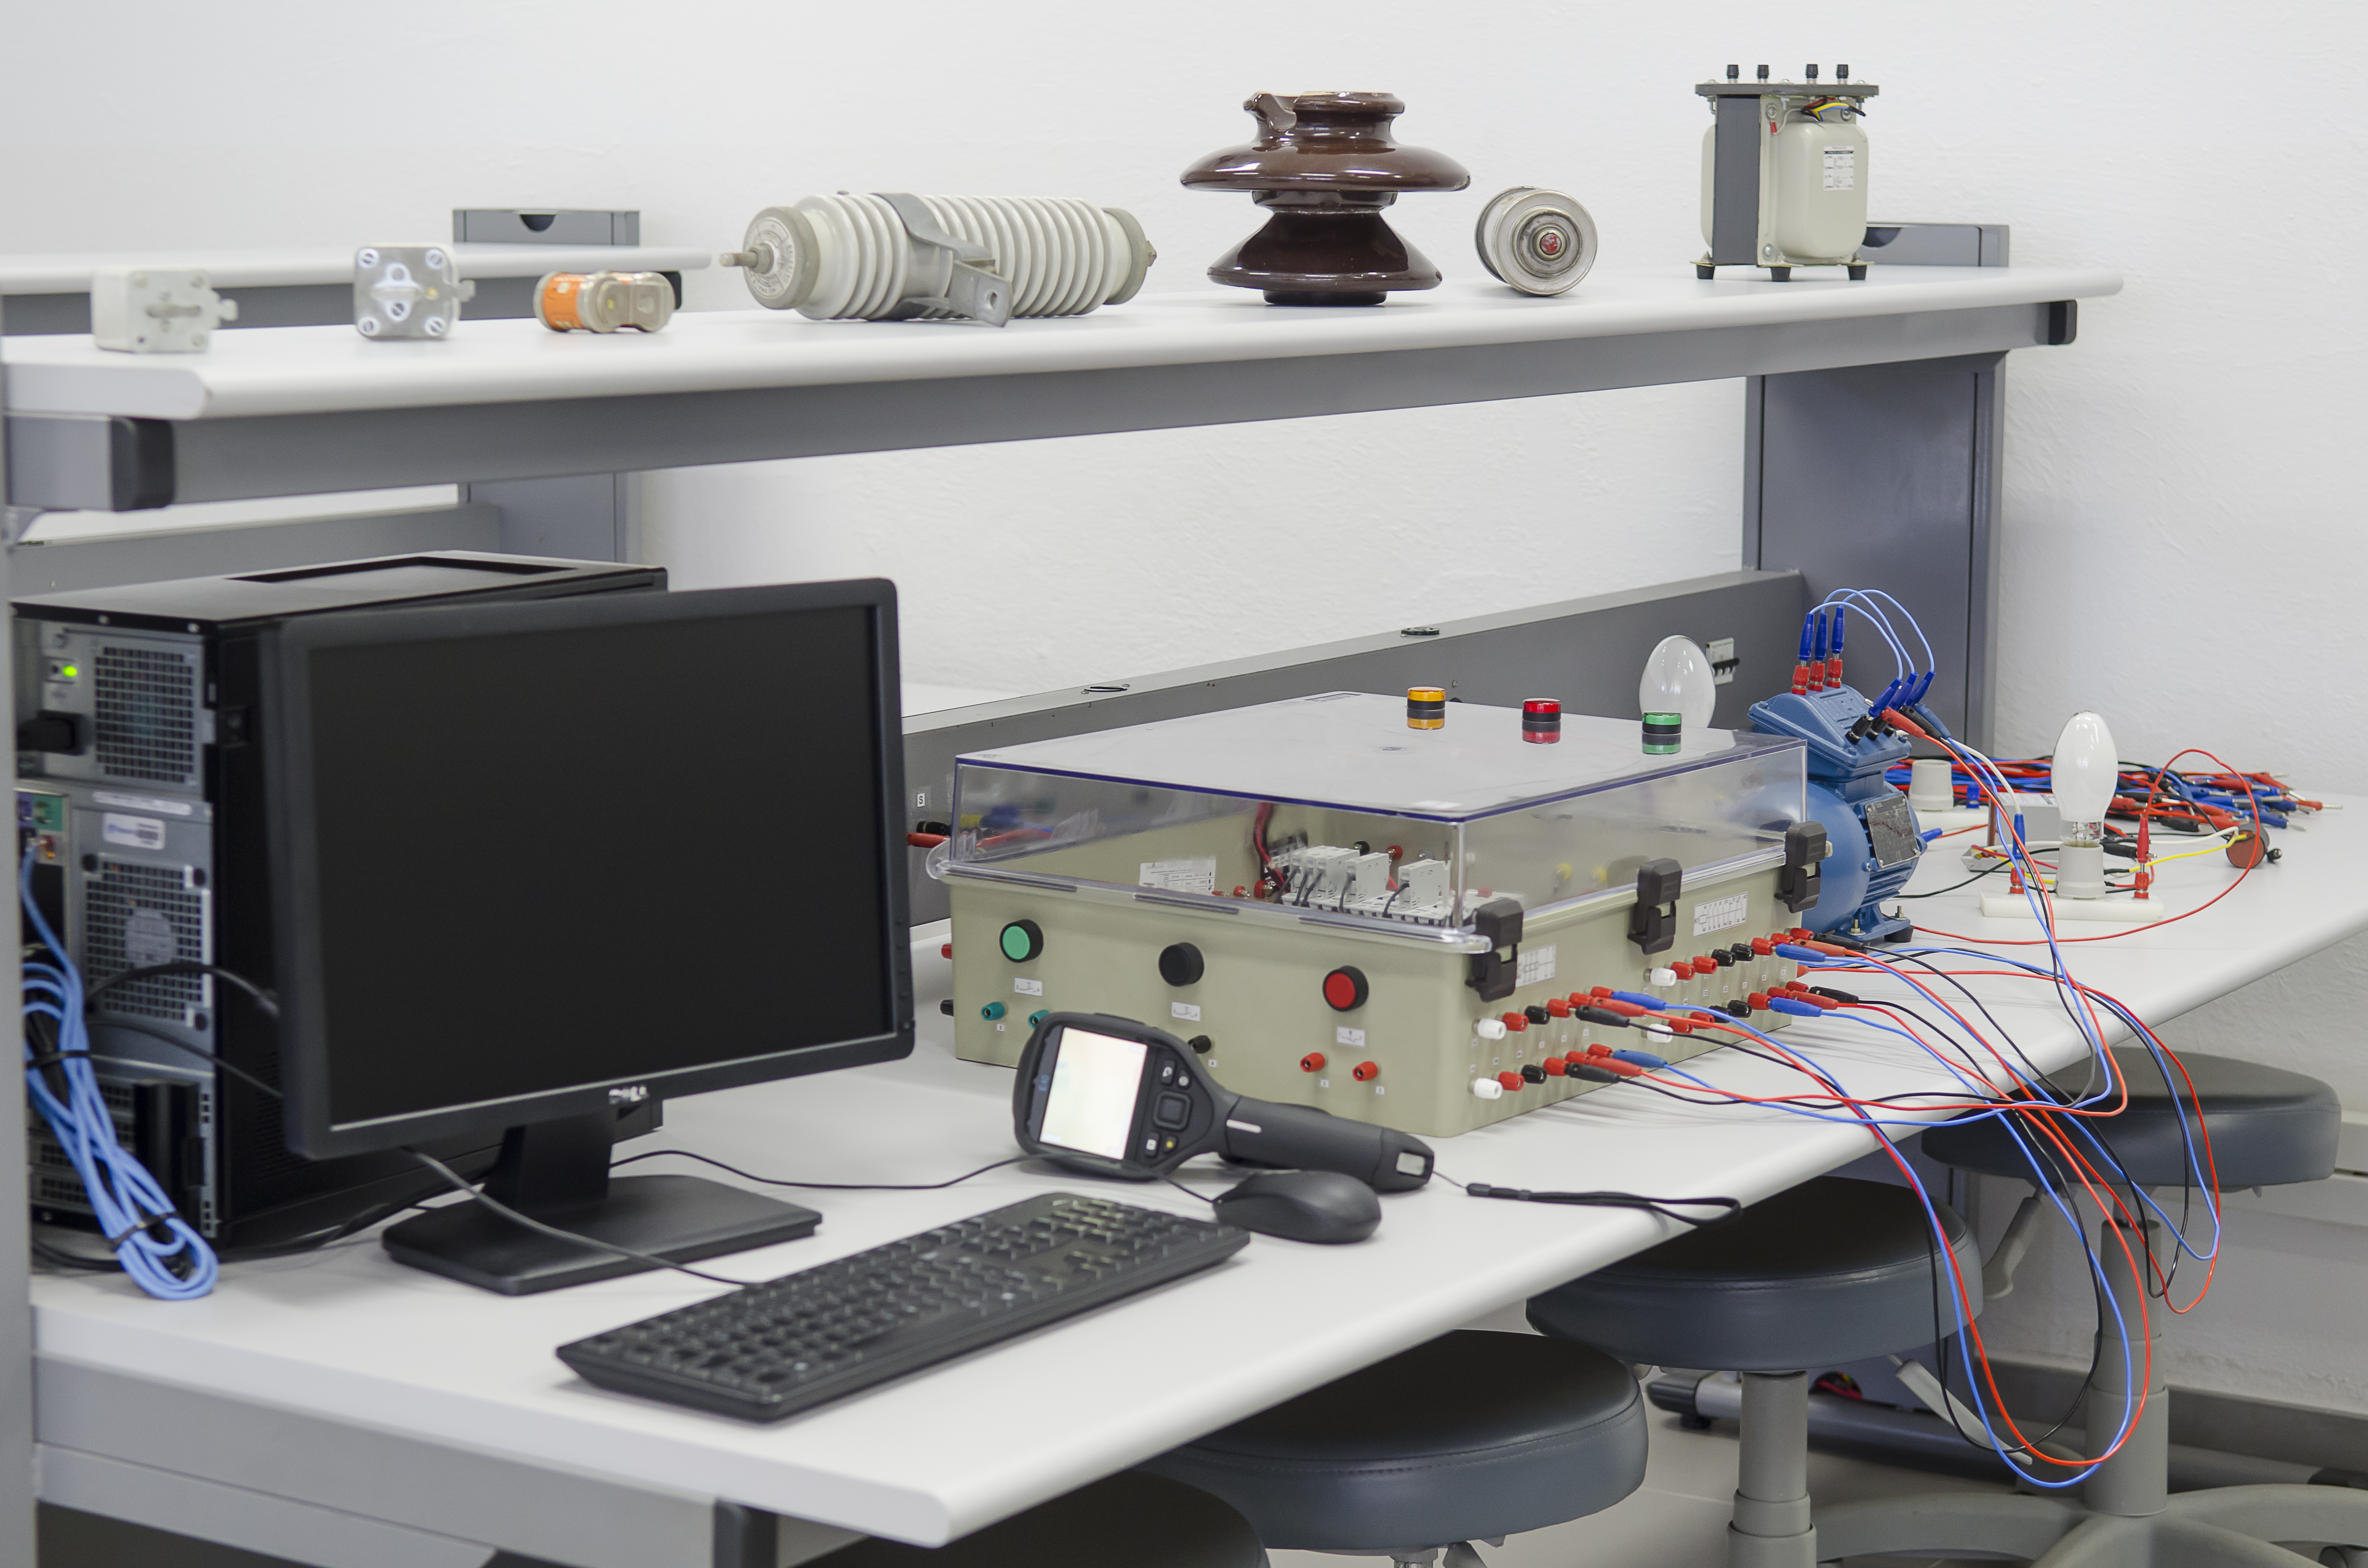
\includegraphics[scale=0.3]{eletrica}
	\end{center}
\end{figure}

O Laboratório de Elétrica é o prédio ao qual está destinado o aprendizado de matérias relacionadas a elétrica, sendo equipada com um braço robótico, diversos tipos de placas de \textit{hardware} acadêmicas e as de uso no mercado de trabalho, lá é possível se utilizar destas ferramentas durante aulas práticas, incrementando o aprendizado dos alunos. Este laboratório não é muito utilizado pelas turmas de Engenharia Civil, apesar de ser aberto para qualquer curso da instituição.

\subsection{Laboratório de Química}

\begin{figure}[htb]
	\caption{\label{fig:quimica} Laboratório de Química}
	\begin{center}
		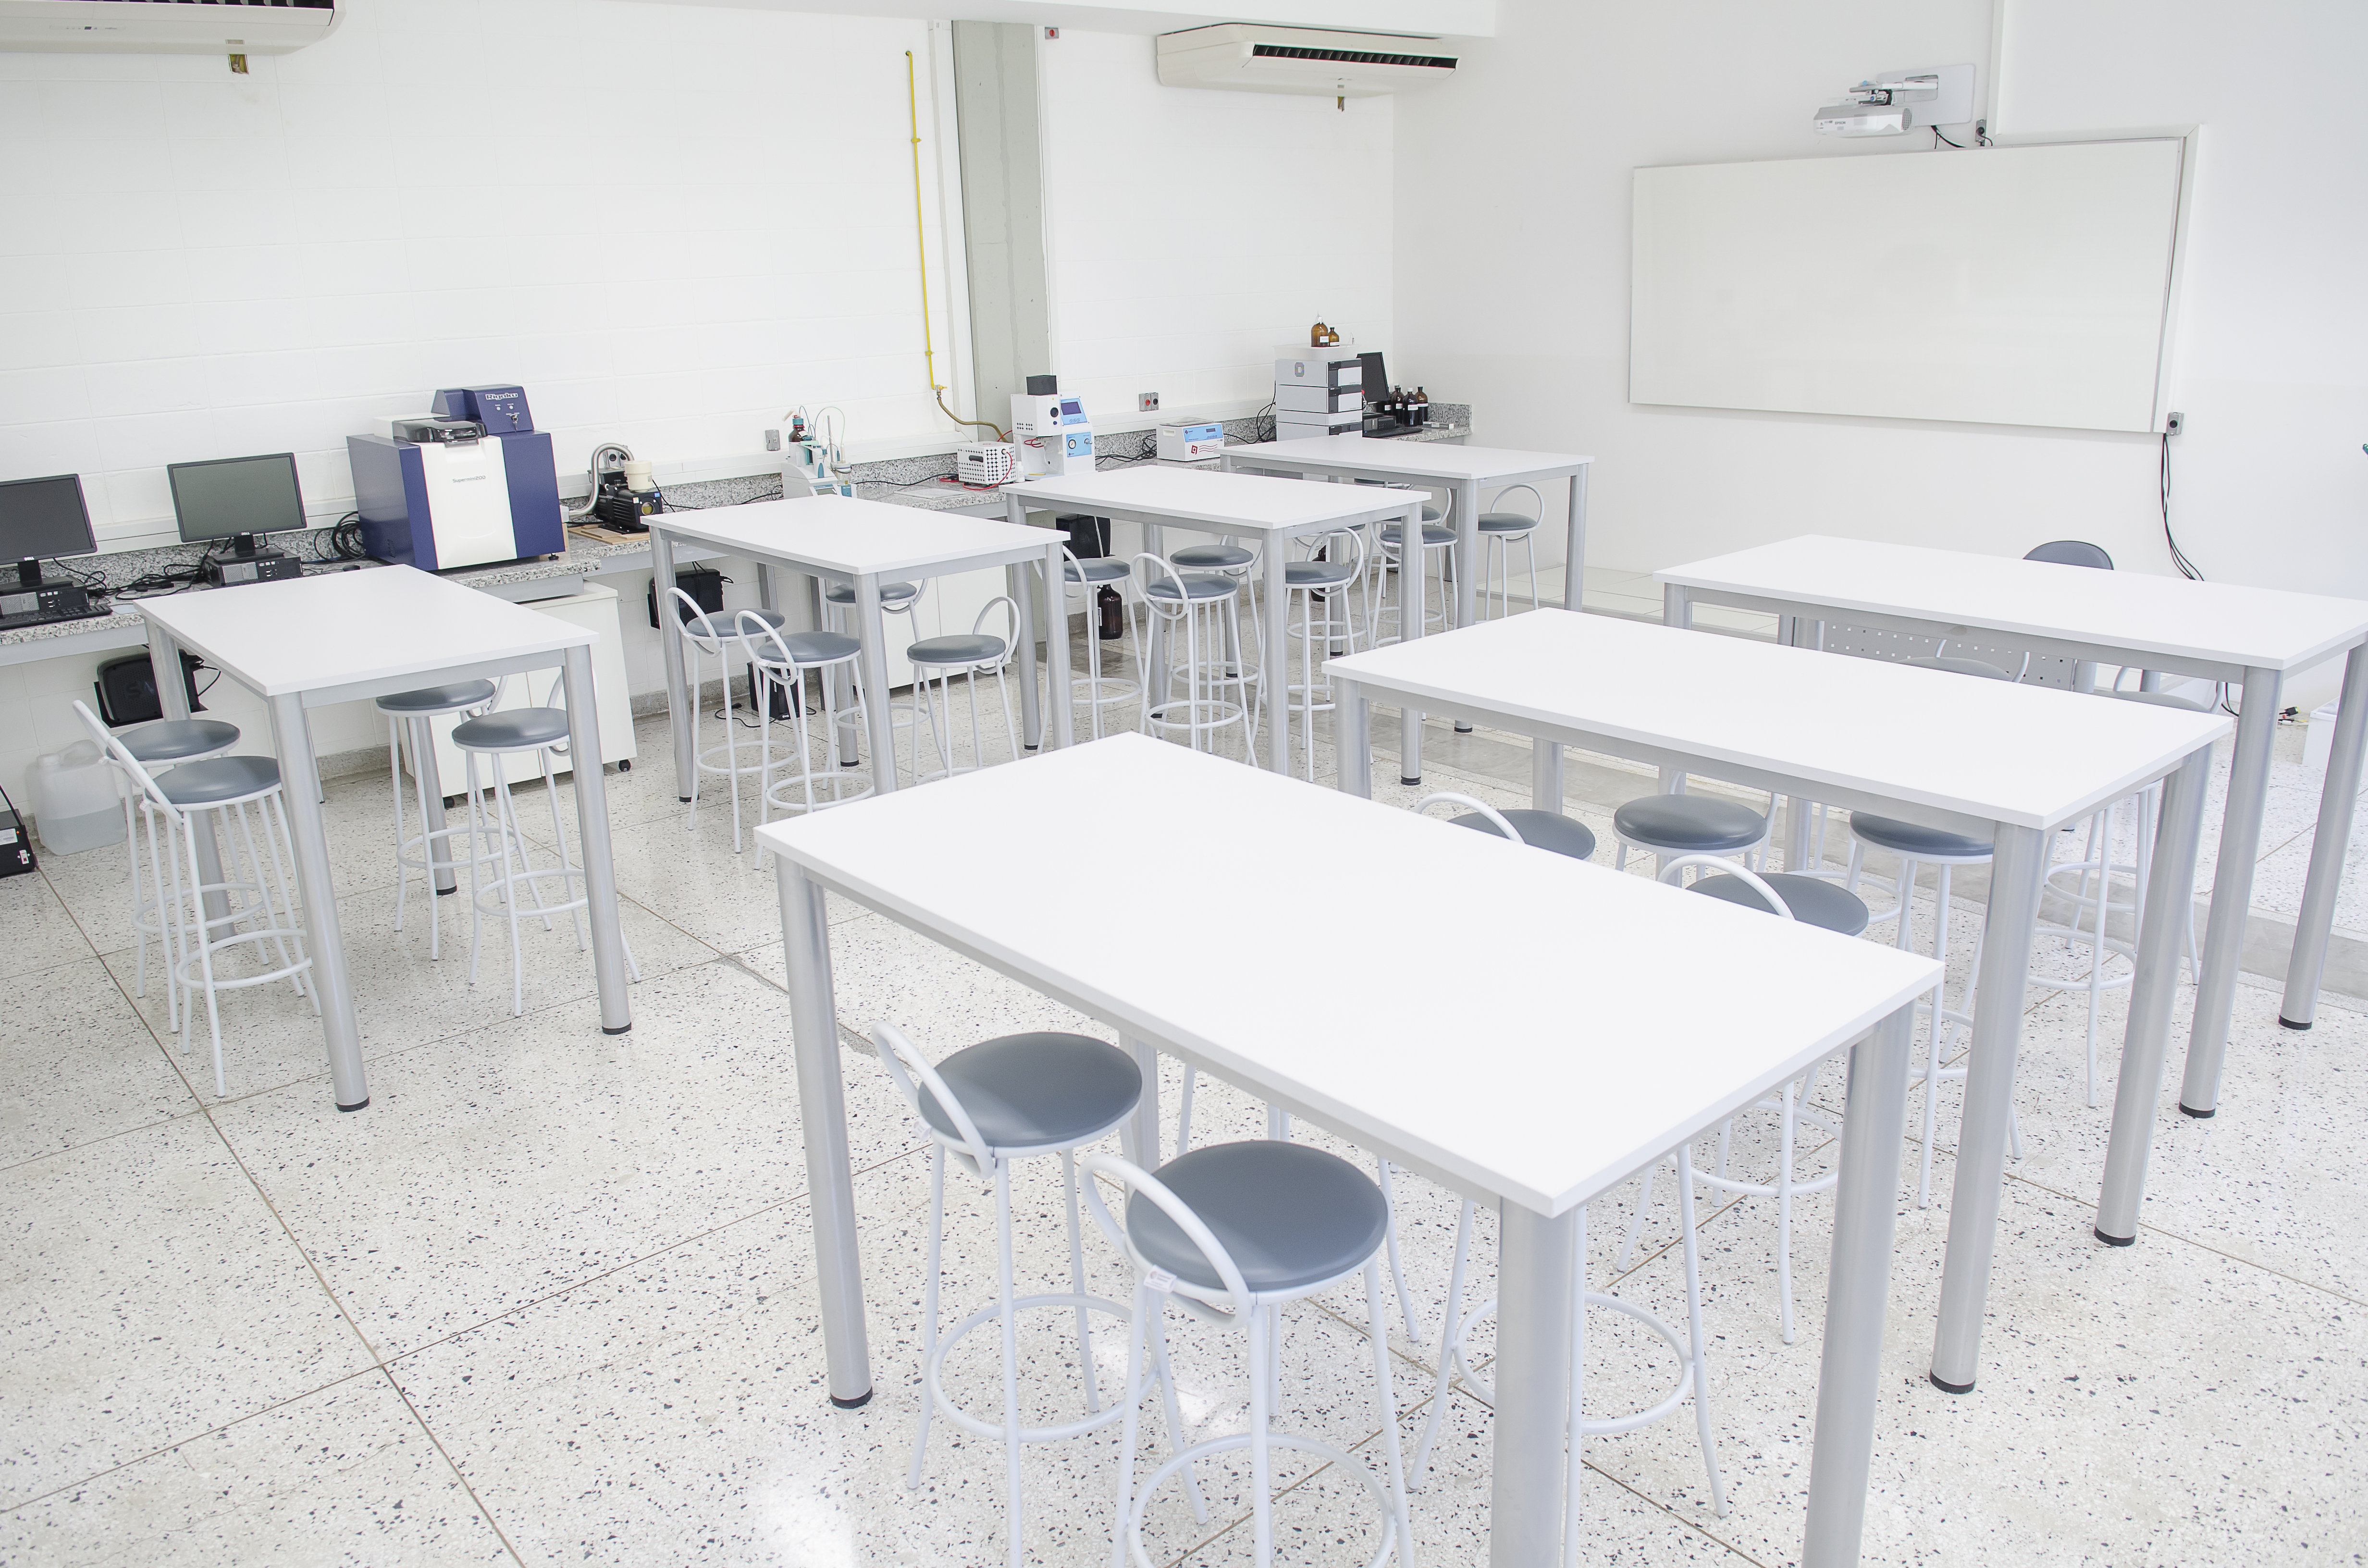
\includegraphics[scale=0.3]{quimica}
	\end{center}
\end{figure}

Este laboratório é destinado em sua maior parte aos alunos dos cursos de Engenharia Química e Engenharia de Alimentos, porém nas disciplinas de química geral, ministradas para as turmas de Computação ele também é usado, equipado com diversas ferramentas como difratômetro, ferramentas de análise de processos, entre outras, proporcionando aos alunos uma grande aprendizagem prática dentro do curso escolhido. Para uso do laboratório é necessário acompanhamento de um professor com horário marcado antecipadamente, devido aos produtos e equipamentos presentes dentro do laboratório.

\subsection{Laboratório de Inovação de Games e Aplicativos}

\begin{figure}[htb]
	\caption{\label{fig:liga} LIGA}
	\begin{center}
		\includegraphics[scale=0.5]{liga}
	\end{center}
\end{figure}

Laboratório destinado ao desenvolvimento de aplicações, android, iOS e jogos educacionais, é conhecido pelo desenvolvimento do aplicativo utilizado por alunos e professores para gestão da vida acadêmica, possui funcionários empregado nos projetos em que atua e também é aberto para a área acadêmica, a fim de apoiar alunos, tanto de Engenharia da Computação, como os de Tecnólogo em Jogos Digitais, no desenvolvimento de seus projetos. Este laboratório é o responsável pela elaboração da Maratona de Desenvolvimento de Jogos, que acontece durante a TecnoFacens, evento de grande prestígio dentro da faculdade, o qual o laboratório é bem engajado, mantendo dentro do seu aplicativo uma área para votação em projetos.

\subsection{Fab Lab}

\begin{figure}[htb]
	\caption{\label{fig:fablab} Fab Lab}
	\begin{center}
		\includegraphics[scale=0.7]{fablab}
	\end{center}
\end{figure}

É um laboratório de prototipagem digital, ou seja, possuem máquinas como CNC de precisão, cortadora a laser, impressora 3D, entre outras máquinas abertas ao publico em geral e empresas parceiras que queiram desenvolver suas ideias lá, em sua maioria são projetos acadêmicos criados por alunos que servem como protótipo para os projetos os quais eles desenvolvem. Frequentemente são realizados \textit{workshops} nos quais são ensinados construção de drones, móveis feitos em MDF, além de treinamentos para operação das máquinas ali presente. Para uso do espaço, é necessário agendamento prévio feito online, e aos sábados o laboratório se mantêm aberto para a comunidade, chamado de dia \textit{Open Day}.

Ele tem ganhado destaque na mídia por ser o primeiro Fab Lab do interior de São Paulo, tendo criado seu próprio sistema de gerenciamento de usuários, o qual está sendo substituído por um projeto \textit{Open Source} originado na França, que tende manter em uma única plataforma todos os projetos cadastrados por todos os Fab Labs do mundo. 

\section{Equipe de Trabalho}

\begin{figure}[htb]
	\caption{\label{fig:equipefacens} Equipe de Trabalho da Facens}
	\begin{center}
		\includegraphics[scale=0.6]{equipefacens}
	\end{center}
\end{figure}

\label{sec:equipetrabalho}
A equipe de trabalho é composta diretamente por sete integrantes, dentre eles, duplas trabalhando em cada frente de responsabilidade do setor.

\subsection{Infraestrutra}
Na frente de infraestrutura se encontra o Renato Bonani e Tiago Barbosa cuidando de servidores, configurações de rede, implementação de controle de acesso, criação e deleção de usuários, além de cuidar de sistema de cancelas e câmeras, sempre estão engajados em novos projetos para a melhoria da infraestrutura dentro da faculdade.

\subsection{Sistemas}
Na frente relacionada a sistemas de gerenciamento de usuários e banco de dados estão Diogo Silva e Lucas Mota, os quais fazem a função de DBA  e cuidam de informações, emissão de relatórios e todos os tipos de integração e administração do sistema Totvs, além de atendimento aos usuários do sistema, sempre estão relacionados a novos projetos, como criação de painéis via PowerBI e implantação de novas versões de sistemas.

\subsection{Desenvolvimento}
Na frente de desenvolvimento estão Alex Coelho e Flávio Bogila, os quais tem a responsabilidade de implementar novos sistemas corporativos e acadêmicos, dar suporte a sistemas legados, geralmente são sistemas vindos de uma demanda interna, apesar de existirem projetos externos a faculdade. É a equipe que mais recebe novos projetos, sendo eles a implantação do Sales Force, sistema de correção de provas, acervo de e-books, entre outros, além de disponibilizar via API dados para aplicações integradas a Faculdade Newton Paiva e ao Laboratório de Inovação e Desenvolvimento de Games e Aplicativos.

\subsection{Gerenciamento}
O setor é gerenciado por Gustavo Monteiro o qual tem a responsabilidade de documentar os projetos desenvolvidos e realizar a gestão do tempo dedicado a cada projeto, além de indicar as ações a serem tomadas em cada ocorrência. É dele também o dever de receber demandas e delegá-las a equipe.

\section{Inter-relação com Outras Áreas da Empresa}
\label{sec:relacaoareas}

O setor de TI, no qual se desenvolveu o estágio sempre está em constante relacionamento com a equipe de outros setores, pois é através de outros setores que se surgem as demandas. De forma direta, até mesmo pela localização do setor, a secretaria que se utiliza de sistemas, como chamada, gerador de provas e o sistema de gestão dos alunos, é um setor que está relacionado ao TI por ser ele quem mantêm as atualizações e manutenções feitas nestes sistemas, desta forma se torna necessário entender das regras de negócio do setor, entender o dia a dia e funcionamento para que as especificações pedidas sejam atendidas.

Outro setor muito próximo do TI é o LIGA, pelo fato de ser o setor que desenvolve os aplicativos com dados de alunos, como o portal e TecnoFacens, é mantida uma relação próxima de sucesso, como é o exemplo da TecnoFacens em que foram unidos esforços para desenvolver o aplicativo e o site para cadastro de projetos, inscrição em maratonas, marcação de presença e avaliação de projetos durante o evento, neste projeto muitas experiências puderam ser trocadas entre as equipes e houve uma proximidade dos setores.

Tesouraria é outro setor que está em constante sincronia com a TI, pois lá ocorrem processamentos de boletos através de sistemas e gestão de alunos pagantes e não pagantes, fazendo com que a TI esteja alinhada para poder gerar boletos ou realizar alterações referentes a pagamentos.

No geral todas as áreas acabam tendo relação com o TI, pois em todos os novos projetos dentro da faculdade que demandem o uso de alguma ferramenta mantida pelo TI, se terá uma relação com esse setor ao qual se está utilizando dos recursos, essa troca de experiência e entendimento das atividades realizadas pelos setores vem a incrementar o aprendizado e a melhor relação dentro do ambiente de trabalho. 

\chapter{Atividades Desenvolvidas}
\label{chap:chap5}

\section{Áreas de Identificação com o Curso}
\label{sec:identcurso}

\chapter{Conclusões}
\label{chap:chap6}
O estágio realizado na FACENS teve grande valor, tanto no aprendizado quanto na experiência obtida a nível profissional. Vários desafios foram enfrentados como dificuldades no desenvolvimento por não ter prática em ambiente profissional. 

A barreira de se adequar ao ambiente profissional e novas linguagens de programação foi logo vencida, já que aprender deve ser uma tarefa fácil para profissionais da área de computação e tecnologia, pois mudanças e atualizações são recorrentes.

O desempenho em determinadas tarefas diárias aprimorou-se conforme ganhou-se a experiência, tanto em tempo quanto em qualidade.  Um profissional que entrasse para realizar as mesmas tarefas, independentemente de sua experiência, teria que aprender o trabalho, mesmo que levasse pouco tempo, mas de qualquer forma teria que conhecer os problemas para aprender as soluções, o que não é nada vantajoso para a empresa, pois gera custos maiores do que manter o profissional. A empresa descrita neste documento valorizou o aprendizado adquirido e manteve o estagiário no quadro de funcionários.

Através desta experiência profissional, foi possível analisar que a prática é conquistada com o tempo e, mesmo com anos de experiência, mudanças de empregos obrigam a aprendermos no novo local. Nenhuma empresa trabalha da mesma forma que a outra e talvez a experiência adquirida não é o bastante para o novo local, portanto um bom profissional deve ser capaz de aprender a todo e a qualquer momento para se adaptar aos novos desafios e não estagnar com os conhecimentos adquiridos.

% ----------------------------------------------------------
% Finaliza a parte no bookmark do PDF
% para que se inicie o bookmark na raiz
% e adiciona espaço de parte no Sumário
% ----------------------------------------------------------
\phantompart

% ---
% Conclusão
% ---
%\chapter{Conclusão}
\label{chap:conclusao}
Concluir sobre o trabalho, apresentar pontos de dificuldades de sua aplicação, pontos a serem melhorados e trabalhos futuros

% ----------------------------------------------------------
% ELEMENTOS PÓS-TEXTUAIS
% ----------------------------------------------------------
\postextual
% ----------------------------------------------------------

% ----------------------------------------------------------
% Referências bibliográficas
% ----------------------------------------------------------
%\bibliography{pos-textuais/bibliografia}


%---------------------------------------------------------------------
% INDICE REMISSIVO
%---------------------------------------------------------------------
%\phantompart
\printindex
%---------------------------------------------------------------------

\end{document}
